\begin{frame}{Depósitos del Tesoro Nacional}
\begin{figure}
\centering
\caption{Depósitos del Tesoro Nacional}
\label{fig:depositos}
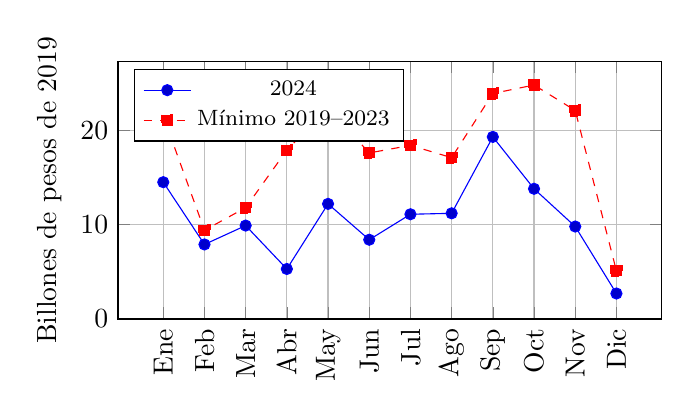
\begin{tikzpicture}
\begin{axis}[
    width=0.7\textwidth,
    height=0.4\textwidth,
    ylabel={Billones de pesos de 2019},
    xtick={1,2,3,4,5,6,7,8,9,10,11,12},
    xticklabels={Ene,Feb,Mar,Abr,May,Jun,Jul,Ago,Sep,Oct,Nov,Dic},
    xticklabel style={rotate=90, anchor=east},
    legend pos=north west,
    grid=both,
    legend style={font=\footnotesize},
    ymin=0
]

% Valores de 2024
\addplot coordinates {
    (1,14.5) (2,7.9) (3,9.9) (4,5.3) (5,12.2) (6,8.4) 
    (7,11.1) (8,11.2) (9,19.3) (10,13.8) (11,9.8) (12,2.7)
};
\addlegendentry{2024}

% Mínimos de 2019 a 2023
\addplot[mark=square*, color=red, dashed] coordinates {
    (1,21.5) (2,9.4) (3,11.8) (4,17.9) (5,22.4) (6,17.6) 
    (7,18.4) (8,17.1) (9,23.9) (10,24.8) (11,22.1) (12,5.1)
};
\addlegendentry{Mínimo 2019--2023}

\end{axis}
\end{tikzpicture}
\vspace{0.1cm}
%\par\footnotesize{\textit{Fuente: Elaboración propia con base en datos de la Dirección de Crédito Público, Ministerio de Hacienda.}}
\end{figure}
\end{frame}
